% Options for packages loaded elsewhere
\PassOptionsToPackage{unicode}{hyperref}
\PassOptionsToPackage{hyphens}{url}
\PassOptionsToPackage{dvipsnames,svgnames,x11names}{xcolor}
%
\documentclass[
  letterpaper,
  DIV=11,
  numbers=noendperiod]{scrartcl}

\usepackage{amsmath,amssymb}
\usepackage{iftex}
\ifPDFTeX
  \usepackage[T1]{fontenc}
  \usepackage[utf8]{inputenc}
  \usepackage{textcomp} % provide euro and other symbols
\else % if luatex or xetex
  \usepackage{unicode-math}
  \defaultfontfeatures{Scale=MatchLowercase}
  \defaultfontfeatures[\rmfamily]{Ligatures=TeX,Scale=1}
\fi
\usepackage{lmodern}
\ifPDFTeX\else  
    % xetex/luatex font selection
\fi
% Use upquote if available, for straight quotes in verbatim environments
\IfFileExists{upquote.sty}{\usepackage{upquote}}{}
\IfFileExists{microtype.sty}{% use microtype if available
  \usepackage[]{microtype}
  \UseMicrotypeSet[protrusion]{basicmath} % disable protrusion for tt fonts
}{}
\makeatletter
\@ifundefined{KOMAClassName}{% if non-KOMA class
  \IfFileExists{parskip.sty}{%
    \usepackage{parskip}
  }{% else
    \setlength{\parindent}{0pt}
    \setlength{\parskip}{6pt plus 2pt minus 1pt}}
}{% if KOMA class
  \KOMAoptions{parskip=half}}
\makeatother
\usepackage{xcolor}
\setlength{\emergencystretch}{3em} % prevent overfull lines
\setcounter{secnumdepth}{-\maxdimen} % remove section numbering
% Make \paragraph and \subparagraph free-standing
\ifx\paragraph\undefined\else
  \let\oldparagraph\paragraph
  \renewcommand{\paragraph}[1]{\oldparagraph{#1}\mbox{}}
\fi
\ifx\subparagraph\undefined\else
  \let\oldsubparagraph\subparagraph
  \renewcommand{\subparagraph}[1]{\oldsubparagraph{#1}\mbox{}}
\fi

\usepackage{color}
\usepackage{fancyvrb}
\newcommand{\VerbBar}{|}
\newcommand{\VERB}{\Verb[commandchars=\\\{\}]}
\DefineVerbatimEnvironment{Highlighting}{Verbatim}{commandchars=\\\{\}}
% Add ',fontsize=\small' for more characters per line
\usepackage{framed}
\definecolor{shadecolor}{RGB}{241,243,245}
\newenvironment{Shaded}{\begin{snugshade}}{\end{snugshade}}
\newcommand{\AlertTok}[1]{\textcolor[rgb]{0.68,0.00,0.00}{#1}}
\newcommand{\AnnotationTok}[1]{\textcolor[rgb]{0.37,0.37,0.37}{#1}}
\newcommand{\AttributeTok}[1]{\textcolor[rgb]{0.40,0.45,0.13}{#1}}
\newcommand{\BaseNTok}[1]{\textcolor[rgb]{0.68,0.00,0.00}{#1}}
\newcommand{\BuiltInTok}[1]{\textcolor[rgb]{0.00,0.23,0.31}{#1}}
\newcommand{\CharTok}[1]{\textcolor[rgb]{0.13,0.47,0.30}{#1}}
\newcommand{\CommentTok}[1]{\textcolor[rgb]{0.37,0.37,0.37}{#1}}
\newcommand{\CommentVarTok}[1]{\textcolor[rgb]{0.37,0.37,0.37}{\textit{#1}}}
\newcommand{\ConstantTok}[1]{\textcolor[rgb]{0.56,0.35,0.01}{#1}}
\newcommand{\ControlFlowTok}[1]{\textcolor[rgb]{0.00,0.23,0.31}{#1}}
\newcommand{\DataTypeTok}[1]{\textcolor[rgb]{0.68,0.00,0.00}{#1}}
\newcommand{\DecValTok}[1]{\textcolor[rgb]{0.68,0.00,0.00}{#1}}
\newcommand{\DocumentationTok}[1]{\textcolor[rgb]{0.37,0.37,0.37}{\textit{#1}}}
\newcommand{\ErrorTok}[1]{\textcolor[rgb]{0.68,0.00,0.00}{#1}}
\newcommand{\ExtensionTok}[1]{\textcolor[rgb]{0.00,0.23,0.31}{#1}}
\newcommand{\FloatTok}[1]{\textcolor[rgb]{0.68,0.00,0.00}{#1}}
\newcommand{\FunctionTok}[1]{\textcolor[rgb]{0.28,0.35,0.67}{#1}}
\newcommand{\ImportTok}[1]{\textcolor[rgb]{0.00,0.46,0.62}{#1}}
\newcommand{\InformationTok}[1]{\textcolor[rgb]{0.37,0.37,0.37}{#1}}
\newcommand{\KeywordTok}[1]{\textcolor[rgb]{0.00,0.23,0.31}{#1}}
\newcommand{\NormalTok}[1]{\textcolor[rgb]{0.00,0.23,0.31}{#1}}
\newcommand{\OperatorTok}[1]{\textcolor[rgb]{0.37,0.37,0.37}{#1}}
\newcommand{\OtherTok}[1]{\textcolor[rgb]{0.00,0.23,0.31}{#1}}
\newcommand{\PreprocessorTok}[1]{\textcolor[rgb]{0.68,0.00,0.00}{#1}}
\newcommand{\RegionMarkerTok}[1]{\textcolor[rgb]{0.00,0.23,0.31}{#1}}
\newcommand{\SpecialCharTok}[1]{\textcolor[rgb]{0.37,0.37,0.37}{#1}}
\newcommand{\SpecialStringTok}[1]{\textcolor[rgb]{0.13,0.47,0.30}{#1}}
\newcommand{\StringTok}[1]{\textcolor[rgb]{0.13,0.47,0.30}{#1}}
\newcommand{\VariableTok}[1]{\textcolor[rgb]{0.07,0.07,0.07}{#1}}
\newcommand{\VerbatimStringTok}[1]{\textcolor[rgb]{0.13,0.47,0.30}{#1}}
\newcommand{\WarningTok}[1]{\textcolor[rgb]{0.37,0.37,0.37}{\textit{#1}}}

\providecommand{\tightlist}{%
  \setlength{\itemsep}{0pt}\setlength{\parskip}{0pt}}\usepackage{longtable,booktabs,array}
\usepackage{calc} % for calculating minipage widths
% Correct order of tables after \paragraph or \subparagraph
\usepackage{etoolbox}
\makeatletter
\patchcmd\longtable{\par}{\if@noskipsec\mbox{}\fi\par}{}{}
\makeatother
% Allow footnotes in longtable head/foot
\IfFileExists{footnotehyper.sty}{\usepackage{footnotehyper}}{\usepackage{footnote}}
\makesavenoteenv{longtable}
\usepackage{graphicx}
\makeatletter
\def\maxwidth{\ifdim\Gin@nat@width>\linewidth\linewidth\else\Gin@nat@width\fi}
\def\maxheight{\ifdim\Gin@nat@height>\textheight\textheight\else\Gin@nat@height\fi}
\makeatother
% Scale images if necessary, so that they will not overflow the page
% margins by default, and it is still possible to overwrite the defaults
% using explicit options in \includegraphics[width, height, ...]{}
\setkeys{Gin}{width=\maxwidth,height=\maxheight,keepaspectratio}
% Set default figure placement to htbp
\makeatletter
\def\fps@figure{htbp}
\makeatother

\KOMAoption{captions}{tableheading}
\makeatletter
\makeatother
\makeatletter
\makeatother
\makeatletter
\@ifpackageloaded{caption}{}{\usepackage{caption}}
\AtBeginDocument{%
\ifdefined\contentsname
  \renewcommand*\contentsname{Table of contents}
\else
  \newcommand\contentsname{Table of contents}
\fi
\ifdefined\listfigurename
  \renewcommand*\listfigurename{List of Figures}
\else
  \newcommand\listfigurename{List of Figures}
\fi
\ifdefined\listtablename
  \renewcommand*\listtablename{List of Tables}
\else
  \newcommand\listtablename{List of Tables}
\fi
\ifdefined\figurename
  \renewcommand*\figurename{Figure}
\else
  \newcommand\figurename{Figure}
\fi
\ifdefined\tablename
  \renewcommand*\tablename{Table}
\else
  \newcommand\tablename{Table}
\fi
}
\@ifpackageloaded{float}{}{\usepackage{float}}
\floatstyle{ruled}
\@ifundefined{c@chapter}{\newfloat{codelisting}{h}{lop}}{\newfloat{codelisting}{h}{lop}[chapter]}
\floatname{codelisting}{Listing}
\newcommand*\listoflistings{\listof{codelisting}{List of Listings}}
\makeatother
\makeatletter
\@ifpackageloaded{caption}{}{\usepackage{caption}}
\@ifpackageloaded{subcaption}{}{\usepackage{subcaption}}
\makeatother
\makeatletter
\@ifpackageloaded{tcolorbox}{}{\usepackage[skins,breakable]{tcolorbox}}
\makeatother
\makeatletter
\@ifundefined{shadecolor}{\definecolor{shadecolor}{rgb}{.97, .97, .97}}
\makeatother
\makeatletter
\makeatother
\makeatletter
\makeatother
\ifLuaTeX
  \usepackage{selnolig}  % disable illegal ligatures
\fi
\IfFileExists{bookmark.sty}{\usepackage{bookmark}}{\usepackage{hyperref}}
\IfFileExists{xurl.sty}{\usepackage{xurl}}{} % add URL line breaks if available
\urlstyle{same} % disable monospaced font for URLs
\hypersetup{
  pdftitle={Class 11},
  pdfauthor={Jesus (A17597539)},
  colorlinks=true,
  linkcolor={blue},
  filecolor={Maroon},
  citecolor={Blue},
  urlcolor={Blue},
  pdfcreator={LaTeX via pandoc}}

\title{Class 11}
\author{Jesus (A17597539)}
\date{}

\begin{document}
\maketitle
\ifdefined\Shaded\renewenvironment{Shaded}{\begin{tcolorbox}[borderline west={3pt}{0pt}{shadecolor}, enhanced, interior hidden, breakable, boxrule=0pt, sharp corners, frame hidden]}{\end{tcolorbox}}\fi

\#PART 1

We need some packages for today's class. These include \texttt{bio3d}
and \texttt{msa}

The \texttt{msa} package id from the BioConductor. These packages focus
on the genomics type work and are managaed by the \texttt{BiocManager}
package.

Install \texttt{install.packages("BiocManager")} and then
\texttt{BiocManager::install("msa")} all entered in the R ``brain''
console

\begin{Shaded}
\begin{Highlighting}[]
\FunctionTok{library}\NormalTok{(bio3d)}

\NormalTok{aa }\OtherTok{\textless{}{-}} \FunctionTok{get.seq}\NormalTok{(}\StringTok{"1ake\_A"}\NormalTok{)}
\end{Highlighting}
\end{Shaded}

\begin{verbatim}
Warning in get.seq("1ake_A"): Removing existing file: seqs.fasta
\end{verbatim}

\begin{verbatim}
Fetching... Please wait. Done.
\end{verbatim}

\begin{Shaded}
\begin{Highlighting}[]
\NormalTok{aa}
\end{Highlighting}
\end{Shaded}

\begin{verbatim}
             1        .         .         .         .         .         60 
pdb|1AKE|A   MRIILLGAPGAGKGTQAQFIMEKYGIPQISTGDMLRAAVKSGSELGKQAKDIMDAGKLVT
             1        .         .         .         .         .         60 

            61        .         .         .         .         .         120 
pdb|1AKE|A   DELVIALVKERIAQEDCRNGFLLDGFPRTIPQADAMKEAGINVDYVLEFDVPDELIVDRI
            61        .         .         .         .         .         120 

           121        .         .         .         .         .         180 
pdb|1AKE|A   VGRRVHAPSGRVYHVKFNPPKVEGKDDVTGEELTTRKDDQEETVRKRLVEYHQMTAPLIG
           121        .         .         .         .         .         180 

           181        .         .         .   214 
pdb|1AKE|A   YYSKEAEAGNTKYAKVDGTKPVAEVRADLEKILG
           181        .         .         .   214 

Call:
  read.fasta(file = outfile)

Class:
  fasta

Alignment dimensions:
  1 sequence rows; 214 position columns (214 non-gap, 0 gap) 

+ attr: id, ali, call
\end{verbatim}

Now I can search the PDB database for related sequences:

\begin{Shaded}
\begin{Highlighting}[]
\CommentTok{\#b \textless{}{-} blast.pdb(aa)}
\end{Highlighting}
\end{Shaded}

\begin{Shaded}
\begin{Highlighting}[]
\CommentTok{\#hits \textless{}{-} plot(b)}
\end{Highlighting}
\end{Shaded}

\begin{Shaded}
\begin{Highlighting}[]
\CommentTok{\#attributes(b)}

\CommentTok{\#head(b$hit.tbl)}
\end{Highlighting}
\end{Shaded}

These are the related structures in the PDB database that we found via a
BLAST search\ldots{}

\begin{Shaded}
\begin{Highlighting}[]
\NormalTok{hits }\OtherTok{\textless{}{-}} \ConstantTok{NULL}
\NormalTok{hits}\SpecialCharTok{$}\NormalTok{pdb.id }\OtherTok{\textless{}{-}} \FunctionTok{c}\NormalTok{(}\StringTok{\textquotesingle{}1AKE\_A\textquotesingle{}}\NormalTok{,}\StringTok{\textquotesingle{}6S36\_A\textquotesingle{}}\NormalTok{,}\StringTok{\textquotesingle{}6RZE\_A\textquotesingle{}}\NormalTok{,}\StringTok{\textquotesingle{}3HPR\_A\textquotesingle{}}\NormalTok{,}\StringTok{\textquotesingle{}1E4V\_A\textquotesingle{}}\NormalTok{,}\StringTok{\textquotesingle{}5EJE\_A\textquotesingle{}}\NormalTok{,}\StringTok{\textquotesingle{}1E4Y\_A\textquotesingle{}}\NormalTok{,}\StringTok{\textquotesingle{}3X2S\_A\textquotesingle{}}\NormalTok{,}\StringTok{\textquotesingle{}6HAP\_A\textquotesingle{}}\NormalTok{,}\StringTok{\textquotesingle{}6HAM\_A\textquotesingle{}}\NormalTok{,}\StringTok{\textquotesingle{}4K46\_A\textquotesingle{}}\NormalTok{,}\StringTok{\textquotesingle{}3GMT\_A\textquotesingle{}}\NormalTok{,}\StringTok{\textquotesingle{}4PZL\_A\textquotesingle{}}\NormalTok{)}
\end{Highlighting}
\end{Shaded}

Side-note: Lets annotate these structures (in other words find out what
they are, what species they are from, stuff about the experiment they
were solved in etc.)

For this we can use the \texttt{pdb.annotate()}

\begin{Shaded}
\begin{Highlighting}[]
\NormalTok{anno }\OtherTok{\textless{}{-}} \FunctionTok{pdb.annotate}\NormalTok{(hits}\SpecialCharTok{$}\NormalTok{pdb.id)}
\end{Highlighting}
\end{Shaded}

\begin{Shaded}
\begin{Highlighting}[]
\FunctionTok{attributes}\NormalTok{(anno)}
\end{Highlighting}
\end{Shaded}

\begin{verbatim}
$names
 [1] "structureId"           "chainId"               "macromoleculeType"    
 [4] "chainLength"           "experimentalTechnique" "resolution"           
 [7] "scopDomain"            "pfam"                  "ligandId"             
[10] "ligandName"            "source"                "structureTitle"       
[13] "citation"              "rObserved"             "rFree"                
[16] "rWork"                 "spaceGroup"           

$class
[1] "data.frame"

$row.names
 [1] "1AKE_A" "6S36_A" "6RZE_A" "3HPR_A" "1E4V_A" "5EJE_A" "1E4Y_A" "3X2S_A"
 [9] "6HAP_A" "6HAM_A" "4K46_A" "3GMT_A" "4PZL_A"
\end{verbatim}

\begin{Shaded}
\begin{Highlighting}[]
\FunctionTok{head}\NormalTok{(anno)}
\end{Highlighting}
\end{Shaded}

\begin{verbatim}
       structureId chainId macromoleculeType chainLength experimentalTechnique
1AKE_A        1AKE       A           Protein         214                 X-ray
6S36_A        6S36       A           Protein         214                 X-ray
6RZE_A        6RZE       A           Protein         214                 X-ray
3HPR_A        3HPR       A           Protein         214                 X-ray
1E4V_A        1E4V       A           Protein         214                 X-ray
5EJE_A        5EJE       A           Protein         214                 X-ray
       resolution       scopDomain                                        pfam
1AKE_A       2.00 Adenylate kinase Adenylate kinase, active site lid (ADK_lid)
6S36_A       1.60             <NA> Adenylate kinase, active site lid (ADK_lid)
6RZE_A       1.69             <NA> Adenylate kinase, active site lid (ADK_lid)
3HPR_A       2.00             <NA> Adenylate kinase, active site lid (ADK_lid)
1E4V_A       1.85 Adenylate kinase Adenylate kinase, active site lid (ADK_lid)
5EJE_A       1.90             <NA> Adenylate kinase, active site lid (ADK_lid)
               ligandId                                       ligandName
1AKE_A              AP5                 BIS(ADENOSINE)-5'-PENTAPHOSPHATE
6S36_A CL (3),NA,MG (2)    CHLORIDE ION (3),SODIUM ION,MAGNESIUM ION (2)
6RZE_A    NA (3),CL (2)                  SODIUM ION (3),CHLORIDE ION (2)
3HPR_A              AP5                 BIS(ADENOSINE)-5'-PENTAPHOSPHATE
1E4V_A              AP5                 BIS(ADENOSINE)-5'-PENTAPHOSPHATE
5EJE_A           AP5,CO BIS(ADENOSINE)-5'-PENTAPHOSPHATE,COBALT (II) ION
                                       source
1AKE_A                       Escherichia coli
6S36_A                       Escherichia coli
6RZE_A                       Escherichia coli
3HPR_A                  Escherichia coli K-12
1E4V_A                       Escherichia coli
5EJE_A Escherichia coli O139:H28 str. E24377A
                                                                                                                                                                     structureTitle
1AKE_A STRUCTURE OF THE COMPLEX BETWEEN ADENYLATE KINASE FROM ESCHERICHIA COLI AND THE INHIBITOR AP5A REFINED AT 1.9 ANGSTROMS RESOLUTION: A MODEL FOR A CATALYTIC TRANSITION STATE
6S36_A                                                                                                                   Crystal structure of E. coli Adenylate kinase R119K mutant
6RZE_A                                                                                                                   Crystal structure of E. coli Adenylate kinase R119A mutant
3HPR_A                                                                                               Crystal structure of V148G adenylate kinase from E. coli, in complex with Ap5A
1E4V_A                                                                                                       Mutant G10V of adenylate kinase from E. coli, modified in the Gly-loop
5EJE_A                                                                                  Crystal structure of E. coli Adenylate kinase G56C/T163C double mutant in complex with Ap5a
                                                    citation rObserved  rFree
1AKE_A                Muller, C.W., et al. J Mol Biol (1992)    0.1960     NA
6S36_A                 Rogne, P., et al. Biochemistry (2019)    0.1632 0.2356
6RZE_A                 Rogne, P., et al. Biochemistry (2019)    0.1865 0.2350
3HPR_A Schrank, T.P., et al. Proc Natl Acad Sci U S A (2009)    0.2100 0.2432
1E4V_A                  Muller, C.W., et al. Proteins (1993)    0.1960     NA
5EJE_A Kovermann, M., et al. Proc Natl Acad Sci U S A (2017)    0.1889 0.2358
        rWork spaceGroup
1AKE_A 0.1960  P 21 2 21
6S36_A 0.1594    C 1 2 1
6RZE_A 0.1819    C 1 2 1
3HPR_A 0.2062  P 21 21 2
1E4V_A 0.1960  P 21 2 21
5EJE_A 0.1863  P 21 2 21
\end{verbatim}

Now we can download all these structures for further analysis with the
\texttt{get.pdb()} function

\begin{Shaded}
\begin{Highlighting}[]
\CommentTok{\# Download releated PDB files}
\NormalTok{files }\OtherTok{\textless{}{-}} \FunctionTok{get.pdb}\NormalTok{(hits}\SpecialCharTok{$}\NormalTok{pdb.id, }\AttributeTok{path=}\StringTok{"pdbs"}\NormalTok{, }\AttributeTok{split=}\ConstantTok{TRUE}\NormalTok{, }\AttributeTok{gzip=}\ConstantTok{TRUE}\NormalTok{)}
\end{Highlighting}
\end{Shaded}

\begin{verbatim}
Warning in get.pdb(hits$pdb.id, path = "pdbs", split = TRUE, gzip = TRUE):
pdbs/1AKE.pdb.gz exists. Skipping download
\end{verbatim}

\begin{verbatim}
Warning in get.pdb(hits$pdb.id, path = "pdbs", split = TRUE, gzip = TRUE):
pdbs/6S36.pdb.gz exists. Skipping download
\end{verbatim}

\begin{verbatim}
Warning in get.pdb(hits$pdb.id, path = "pdbs", split = TRUE, gzip = TRUE):
pdbs/6RZE.pdb.gz exists. Skipping download
\end{verbatim}

\begin{verbatim}
Warning in get.pdb(hits$pdb.id, path = "pdbs", split = TRUE, gzip = TRUE):
pdbs/3HPR.pdb.gz exists. Skipping download
\end{verbatim}

\begin{verbatim}
Warning in get.pdb(hits$pdb.id, path = "pdbs", split = TRUE, gzip = TRUE):
pdbs/1E4V.pdb.gz exists. Skipping download
\end{verbatim}

\begin{verbatim}
Warning in get.pdb(hits$pdb.id, path = "pdbs", split = TRUE, gzip = TRUE):
pdbs/5EJE.pdb.gz exists. Skipping download
\end{verbatim}

\begin{verbatim}
Warning in get.pdb(hits$pdb.id, path = "pdbs", split = TRUE, gzip = TRUE):
pdbs/1E4Y.pdb.gz exists. Skipping download
\end{verbatim}

\begin{verbatim}
Warning in get.pdb(hits$pdb.id, path = "pdbs", split = TRUE, gzip = TRUE):
pdbs/3X2S.pdb.gz exists. Skipping download
\end{verbatim}

\begin{verbatim}
Warning in get.pdb(hits$pdb.id, path = "pdbs", split = TRUE, gzip = TRUE):
pdbs/6HAP.pdb.gz exists. Skipping download
\end{verbatim}

\begin{verbatim}
Warning in get.pdb(hits$pdb.id, path = "pdbs", split = TRUE, gzip = TRUE):
pdbs/6HAM.pdb.gz exists. Skipping download
\end{verbatim}

\begin{verbatim}
Warning in get.pdb(hits$pdb.id, path = "pdbs", split = TRUE, gzip = TRUE):
pdbs/4K46.pdb.gz exists. Skipping download
\end{verbatim}

\begin{verbatim}
Warning in get.pdb(hits$pdb.id, path = "pdbs", split = TRUE, gzip = TRUE):
pdbs/3GMT.pdb.gz exists. Skipping download
\end{verbatim}

\begin{verbatim}
Warning in get.pdb(hits$pdb.id, path = "pdbs", split = TRUE, gzip = TRUE):
pdbs/4PZL.pdb.gz exists. Skipping download
\end{verbatim}

\begin{verbatim}

  |                                                                            
  |                                                                      |   0%
  |                                                                            
  |=====                                                                 |   8%
  |                                                                            
  |===========                                                           |  15%
  |                                                                            
  |================                                                      |  23%
  |                                                                            
  |======================                                                |  31%
  |                                                                            
  |===========================                                           |  38%
  |                                                                            
  |================================                                      |  46%
  |                                                                            
  |======================================                                |  54%
  |                                                                            
  |===========================================                           |  62%
  |                                                                            
  |================================================                      |  69%
  |                                                                            
  |======================================================                |  77%
  |                                                                            
  |===========================================================           |  85%
  |                                                                            
  |=================================================================     |  92%
  |                                                                            
  |======================================================================| 100%
\end{verbatim}

Now we have all these related structures we can align and
Superpose\ldots{}

\begin{Shaded}
\begin{Highlighting}[]
\CommentTok{\# Align releated PDBs}
\NormalTok{pdbs }\OtherTok{\textless{}{-}} \FunctionTok{pdbaln}\NormalTok{(files, }\AttributeTok{fit =} \ConstantTok{TRUE}\NormalTok{, }\AttributeTok{exefile=}\StringTok{"msa"}\NormalTok{)}
\end{Highlighting}
\end{Shaded}

\begin{verbatim}
Reading PDB files:
pdbs/split_chain/1AKE_A.pdb
pdbs/split_chain/6S36_A.pdb
pdbs/split_chain/6RZE_A.pdb
pdbs/split_chain/3HPR_A.pdb
pdbs/split_chain/1E4V_A.pdb
pdbs/split_chain/5EJE_A.pdb
pdbs/split_chain/1E4Y_A.pdb
pdbs/split_chain/3X2S_A.pdb
pdbs/split_chain/6HAP_A.pdb
pdbs/split_chain/6HAM_A.pdb
pdbs/split_chain/4K46_A.pdb
pdbs/split_chain/3GMT_A.pdb
pdbs/split_chain/4PZL_A.pdb
   PDB has ALT records, taking A only, rm.alt=TRUE
.   PDB has ALT records, taking A only, rm.alt=TRUE
.   PDB has ALT records, taking A only, rm.alt=TRUE
.   PDB has ALT records, taking A only, rm.alt=TRUE
..   PDB has ALT records, taking A only, rm.alt=TRUE
....   PDB has ALT records, taking A only, rm.alt=TRUE
.   PDB has ALT records, taking A only, rm.alt=TRUE
...

Extracting sequences

pdb/seq: 1   name: pdbs/split_chain/1AKE_A.pdb 
   PDB has ALT records, taking A only, rm.alt=TRUE
pdb/seq: 2   name: pdbs/split_chain/6S36_A.pdb 
   PDB has ALT records, taking A only, rm.alt=TRUE
pdb/seq: 3   name: pdbs/split_chain/6RZE_A.pdb 
   PDB has ALT records, taking A only, rm.alt=TRUE
pdb/seq: 4   name: pdbs/split_chain/3HPR_A.pdb 
   PDB has ALT records, taking A only, rm.alt=TRUE
pdb/seq: 5   name: pdbs/split_chain/1E4V_A.pdb 
pdb/seq: 6   name: pdbs/split_chain/5EJE_A.pdb 
   PDB has ALT records, taking A only, rm.alt=TRUE
pdb/seq: 7   name: pdbs/split_chain/1E4Y_A.pdb 
pdb/seq: 8   name: pdbs/split_chain/3X2S_A.pdb 
pdb/seq: 9   name: pdbs/split_chain/6HAP_A.pdb 
pdb/seq: 10   name: pdbs/split_chain/6HAM_A.pdb 
   PDB has ALT records, taking A only, rm.alt=TRUE
pdb/seq: 11   name: pdbs/split_chain/4K46_A.pdb 
   PDB has ALT records, taking A only, rm.alt=TRUE
pdb/seq: 12   name: pdbs/split_chain/3GMT_A.pdb 
pdb/seq: 13   name: pdbs/split_chain/4PZL_A.pdb 
\end{verbatim}

\begin{Shaded}
\begin{Highlighting}[]
\NormalTok{pdbs}
\end{Highlighting}
\end{Shaded}

\begin{verbatim}
                                1        .         .         .         40 
[Truncated_Name:1]1AKE_A.pdb    ----------MRIILLGAPGAGKGTQAQFIMEKYGIPQIS
[Truncated_Name:2]6S36_A.pdb    ----------MRIILLGAPGAGKGTQAQFIMEKYGIPQIS
[Truncated_Name:3]6RZE_A.pdb    ----------MRIILLGAPGAGKGTQAQFIMEKYGIPQIS
[Truncated_Name:4]3HPR_A.pdb    ----------MRIILLGAPGAGKGTQAQFIMEKYGIPQIS
[Truncated_Name:5]1E4V_A.pdb    ----------MRIILLGAPVAGKGTQAQFIMEKYGIPQIS
[Truncated_Name:6]5EJE_A.pdb    ----------MRIILLGAPGAGKGTQAQFIMEKYGIPQIS
[Truncated_Name:7]1E4Y_A.pdb    ----------MRIILLGALVAGKGTQAQFIMEKYGIPQIS
[Truncated_Name:8]3X2S_A.pdb    ----------MRIILLGAPGAGKGTQAQFIMEKYGIPQIS
[Truncated_Name:9]6HAP_A.pdb    ----------MRIILLGAPGAGKGTQAQFIMEKYGIPQIS
[Truncated_Name:10]6HAM_A.pdb   ----------MRIILLGAPGAGKGTQAQFIMEKYGIPQIS
[Truncated_Name:11]4K46_A.pdb   ----------MRIILLGAPGAGKGTQAQFIMAKFGIPQIS
[Truncated_Name:12]3GMT_A.pdb   ----------MRLILLGAPGAGKGTQANFIKEKFGIPQIS
[Truncated_Name:13]4PZL_A.pdb   TENLYFQSNAMRIILLGAPGAGKGTQAKIIEQKYNIAHIS
                                          **^*****  *******  *  *^ *  ** 
                                1        .         .         .         40 

                               41        .         .         .         80 
[Truncated_Name:1]1AKE_A.pdb    TGDMLRAAVKSGSELGKQAKDIMDAGKLVTDELVIALVKE
[Truncated_Name:2]6S36_A.pdb    TGDMLRAAVKSGSELGKQAKDIMDAGKLVTDELVIALVKE
[Truncated_Name:3]6RZE_A.pdb    TGDMLRAAVKSGSELGKQAKDIMDAGKLVTDELVIALVKE
[Truncated_Name:4]3HPR_A.pdb    TGDMLRAAVKSGSELGKQAKDIMDAGKLVTDELVIALVKE
[Truncated_Name:5]1E4V_A.pdb    TGDMLRAAVKSGSELGKQAKDIMDAGKLVTDELVIALVKE
[Truncated_Name:6]5EJE_A.pdb    TGDMLRAAVKSGSELGKQAKDIMDACKLVTDELVIALVKE
[Truncated_Name:7]1E4Y_A.pdb    TGDMLRAAVKSGSELGKQAKDIMDAGKLVTDELVIALVKE
[Truncated_Name:8]3X2S_A.pdb    TGDMLRAAVKSGSELGKQAKDIMDCGKLVTDELVIALVKE
[Truncated_Name:9]6HAP_A.pdb    TGDMLRAAVKSGSELGKQAKDIMDAGKLVTDELVIALVRE
[Truncated_Name:10]6HAM_A.pdb   TGDMLRAAIKSGSELGKQAKDIMDAGKLVTDEIIIALVKE
[Truncated_Name:11]4K46_A.pdb   TGDMLRAAIKAGTELGKQAKSVIDAGQLVSDDIILGLVKE
[Truncated_Name:12]3GMT_A.pdb   TGDMLRAAVKAGTPLGVEAKTYMDEGKLVPDSLIIGLVKE
[Truncated_Name:13]4PZL_A.pdb   TGDMIRETIKSGSALGQELKKVLDAGELVSDEFIIKIVKD
                                ****^*  ^* *^ **   *  ^*   ** *  ^^ ^*^^ 
                               41        .         .         .         80 

                               81        .         .         .         120 
[Truncated_Name:1]1AKE_A.pdb    RIAQEDCRNGFLLDGFPRTIPQADAMKEAGINVDYVLEFD
[Truncated_Name:2]6S36_A.pdb    RIAQEDCRNGFLLDGFPRTIPQADAMKEAGINVDYVLEFD
[Truncated_Name:3]6RZE_A.pdb    RIAQEDCRNGFLLDGFPRTIPQADAMKEAGINVDYVLEFD
[Truncated_Name:4]3HPR_A.pdb    RIAQEDCRNGFLLDGFPRTIPQADAMKEAGINVDYVLEFD
[Truncated_Name:5]1E4V_A.pdb    RIAQEDCRNGFLLDGFPRTIPQADAMKEAGINVDYVLEFD
[Truncated_Name:6]5EJE_A.pdb    RIAQEDCRNGFLLDGFPRTIPQADAMKEAGINVDYVLEFD
[Truncated_Name:7]1E4Y_A.pdb    RIAQEDCRNGFLLDGFPRTIPQADAMKEAGINVDYVLEFD
[Truncated_Name:8]3X2S_A.pdb    RIAQEDSRNGFLLDGFPRTIPQADAMKEAGINVDYVLEFD
[Truncated_Name:9]6HAP_A.pdb    RICQEDSRNGFLLDGFPRTIPQADAMKEAGINVDYVLEFD
[Truncated_Name:10]6HAM_A.pdb   RICQEDSRNGFLLDGFPRTIPQADAMKEAGINVDYVLEFD
[Truncated_Name:11]4K46_A.pdb   RIAQDDCAKGFLLDGFPRTIPQADGLKEVGVVVDYVIEFD
[Truncated_Name:12]3GMT_A.pdb   RLKEADCANGYLFDGFPRTIAQADAMKEAGVAIDYVLEID
[Truncated_Name:13]4PZL_A.pdb   RISKNDCNNGFLLDGVPRTIPQAQELDKLGVNIDYIVEVD
                                *^   *   *^* ** **** **  ^   *^ ^**^^* * 
                               81        .         .         .         120 

                              121        .         .         .         160 
[Truncated_Name:1]1AKE_A.pdb    VPDELIVDRIVGRRVHAPSGRVYHVKFNPPKVEGKDDVTG
[Truncated_Name:2]6S36_A.pdb    VPDELIVDKIVGRRVHAPSGRVYHVKFNPPKVEGKDDVTG
[Truncated_Name:3]6RZE_A.pdb    VPDELIVDAIVGRRVHAPSGRVYHVKFNPPKVEGKDDVTG
[Truncated_Name:4]3HPR_A.pdb    VPDELIVDRIVGRRVHAPSGRVYHVKFNPPKVEGKDDGTG
[Truncated_Name:5]1E4V_A.pdb    VPDELIVDRIVGRRVHAPSGRVYHVKFNPPKVEGKDDVTG
[Truncated_Name:6]5EJE_A.pdb    VPDELIVDRIVGRRVHAPSGRVYHVKFNPPKVEGKDDVTG
[Truncated_Name:7]1E4Y_A.pdb    VPDELIVDRIVGRRVHAPSGRVYHVKFNPPKVEGKDDVTG
[Truncated_Name:8]3X2S_A.pdb    VPDELIVDRIVGRRVHAPSGRVYHVKFNPPKVEGKDDVTG
[Truncated_Name:9]6HAP_A.pdb    VPDELIVDRIVGRRVHAPSGRVYHVKFNPPKVEGKDDVTG
[Truncated_Name:10]6HAM_A.pdb   VPDELIVDRIVGRRVHAPSGRVYHVKFNPPKVEGKDDVTG
[Truncated_Name:11]4K46_A.pdb   VADSVIVERMAGRRAHLASGRTYHNVYNPPKVEGKDDVTG
[Truncated_Name:12]3GMT_A.pdb   VPFSEIIERMSGRRTHPASGRTYHVKFNPPKVEGKDDVTG
[Truncated_Name:13]4PZL_A.pdb   VADNLLIERITGRRIHPASGRTYHTKFNPPKVADKDDVTG
                                *    ^^^ ^ *** *  *** **  ^*****  *** ** 
                              121        .         .         .         160 

                              161        .         .         .         200 
[Truncated_Name:1]1AKE_A.pdb    EELTTRKDDQEETVRKRLVEYHQMTAPLIGYYSKEAEAGN
[Truncated_Name:2]6S36_A.pdb    EELTTRKDDQEETVRKRLVEYHQMTAPLIGYYSKEAEAGN
[Truncated_Name:3]6RZE_A.pdb    EELTTRKDDQEETVRKRLVEYHQMTAPLIGYYSKEAEAGN
[Truncated_Name:4]3HPR_A.pdb    EELTTRKDDQEETVRKRLVEYHQMTAPLIGYYSKEAEAGN
[Truncated_Name:5]1E4V_A.pdb    EELTTRKDDQEETVRKRLVEYHQMTAPLIGYYSKEAEAGN
[Truncated_Name:6]5EJE_A.pdb    EELTTRKDDQEECVRKRLVEYHQMTAPLIGYYSKEAEAGN
[Truncated_Name:7]1E4Y_A.pdb    EELTTRKDDQEETVRKRLVEYHQMTAPLIGYYSKEAEAGN
[Truncated_Name:8]3X2S_A.pdb    EELTTRKDDQEETVRKRLCEYHQMTAPLIGYYSKEAEAGN
[Truncated_Name:9]6HAP_A.pdb    EELTTRKDDQEETVRKRLVEYHQMTAPLIGYYSKEAEAGN
[Truncated_Name:10]6HAM_A.pdb   EELTTRKDDQEETVRKRLVEYHQMTAPLIGYYSKEAEAGN
[Truncated_Name:11]4K46_A.pdb   EDLVIREDDKEETVLARLGVYHNQTAPLIAYYGKEAEAGN
[Truncated_Name:12]3GMT_A.pdb   EPLVQRDDDKEETVKKRLDVYEAQTKPLITYYGDWARRGA
[Truncated_Name:13]4PZL_A.pdb   EPLITRTDDNEDTVKQRLSVYHAQTAKLIDFYRNFSSTNT
                                * *  * ** *^ *  **  *   *  ** ^*         
                              161        .         .         .         200 

                              201        .         .      227 
[Truncated_Name:1]1AKE_A.pdb    T--KYAKVDGTKPVAEVRADLEKILG-
[Truncated_Name:2]6S36_A.pdb    T--KYAKVDGTKPVAEVRADLEKILG-
[Truncated_Name:3]6RZE_A.pdb    T--KYAKVDGTKPVAEVRADLEKILG-
[Truncated_Name:4]3HPR_A.pdb    T--KYAKVDGTKPVAEVRADLEKILG-
[Truncated_Name:5]1E4V_A.pdb    T--KYAKVDGTKPVAEVRADLEKILG-
[Truncated_Name:6]5EJE_A.pdb    T--KYAKVDGTKPVAEVRADLEKILG-
[Truncated_Name:7]1E4Y_A.pdb    T--KYAKVDGTKPVAEVRADLEKILG-
[Truncated_Name:8]3X2S_A.pdb    T--KYAKVDGTKPVAEVRADLEKILG-
[Truncated_Name:9]6HAP_A.pdb    T--KYAKVDGTKPVCEVRADLEKILG-
[Truncated_Name:10]6HAM_A.pdb   T--KYAKVDGTKPVCEVRADLEKILG-
[Truncated_Name:11]4K46_A.pdb   T--QYLKFDGTKAVAEVSAELEKALA-
[Truncated_Name:12]3GMT_A.pdb   E-------NGLKAPA-----YRKISG-
[Truncated_Name:13]4PZL_A.pdb   KIPKYIKINGDQAVEKVSQDIFDQLNK
                                         *                  
                              201        .         .      227 

Call:
  pdbaln(files = files, fit = TRUE, exefile = "msa")

Class:
  pdbs, fasta

Alignment dimensions:
  13 sequence rows; 227 position columns (204 non-gap, 23 gap) 

+ attr: xyz, resno, b, chain, id, ali, resid, sse, call
\end{verbatim}

\begin{Shaded}
\begin{Highlighting}[]
\CommentTok{\# Vector containing PDB codes for figure axis}
\NormalTok{ids }\OtherTok{\textless{}{-}} \FunctionTok{basename.pdb}\NormalTok{(pdbs}\SpecialCharTok{$}\NormalTok{id)}

\CommentTok{\# Draw schematic alignment}
\CommentTok{\#plot(pdbs, labels=ids)}
\end{Highlighting}
\end{Shaded}

\#\#Principal Component Analysis

\begin{Shaded}
\begin{Highlighting}[]
\CommentTok{\# Perform PCA}
\NormalTok{pc.xray }\OtherTok{\textless{}{-}} \FunctionTok{pca}\NormalTok{(pdbs)}
\FunctionTok{plot}\NormalTok{(pc.xray)}
\end{Highlighting}
\end{Shaded}

\begin{figure}[H]

{\centering 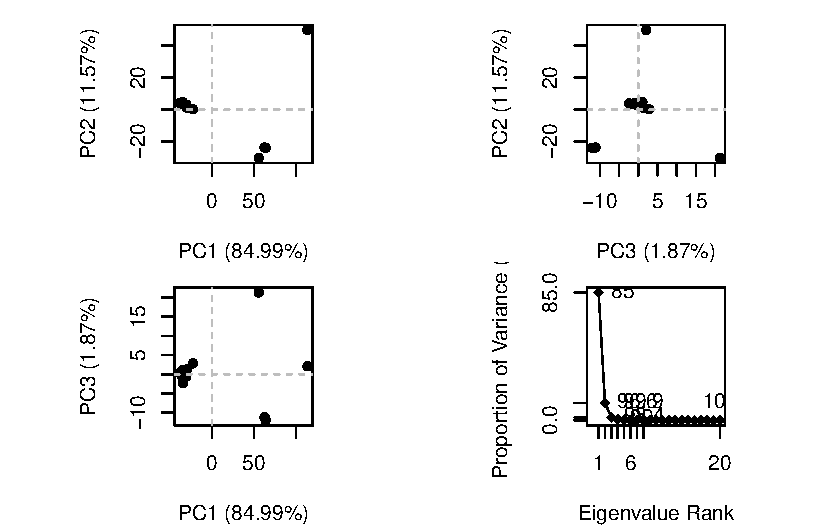
\includegraphics{Class11INCLASS_files/figure-pdf/unnamed-chunk-11-1.pdf}

}

\end{figure}

\begin{Shaded}
\begin{Highlighting}[]
\CommentTok{\# Visualize first principal component}
\NormalTok{pc1 }\OtherTok{\textless{}{-}} \FunctionTok{mktrj}\NormalTok{(pc.xray, }\AttributeTok{pc=}\DecValTok{1}\NormalTok{, }\AttributeTok{file=}\StringTok{"pc\_1.pdb"}\NormalTok{)}
\end{Highlighting}
\end{Shaded}

And a nicer PC plot

\begin{Shaded}
\begin{Highlighting}[]
\CommentTok{\# Calculate RMSD}
\NormalTok{rd }\OtherTok{\textless{}{-}} \FunctionTok{rmsd}\NormalTok{(pdbs)}
\end{Highlighting}
\end{Shaded}

\begin{verbatim}
Warning in rmsd(pdbs): No indices provided, using the 204 non NA positions
\end{verbatim}

\begin{Shaded}
\begin{Highlighting}[]
\CommentTok{\# Structure{-}based clustering}
\NormalTok{hc.rd }\OtherTok{\textless{}{-}} \FunctionTok{hclust}\NormalTok{(}\FunctionTok{dist}\NormalTok{(rd))}
\NormalTok{grps.rd }\OtherTok{\textless{}{-}} \FunctionTok{cutree}\NormalTok{(hc.rd, }\AttributeTok{k=}\DecValTok{3}\NormalTok{)}

\FunctionTok{plot}\NormalTok{(pc.xray, }\DecValTok{1}\SpecialCharTok{:}\DecValTok{2}\NormalTok{, }\AttributeTok{col=}\StringTok{"grey50"}\NormalTok{, }\AttributeTok{bg=}\NormalTok{grps.rd, }\AttributeTok{pch=}\DecValTok{21}\NormalTok{, }\AttributeTok{cex=}\DecValTok{1}\NormalTok{)}
\end{Highlighting}
\end{Shaded}

\begin{figure}[H]

{\centering 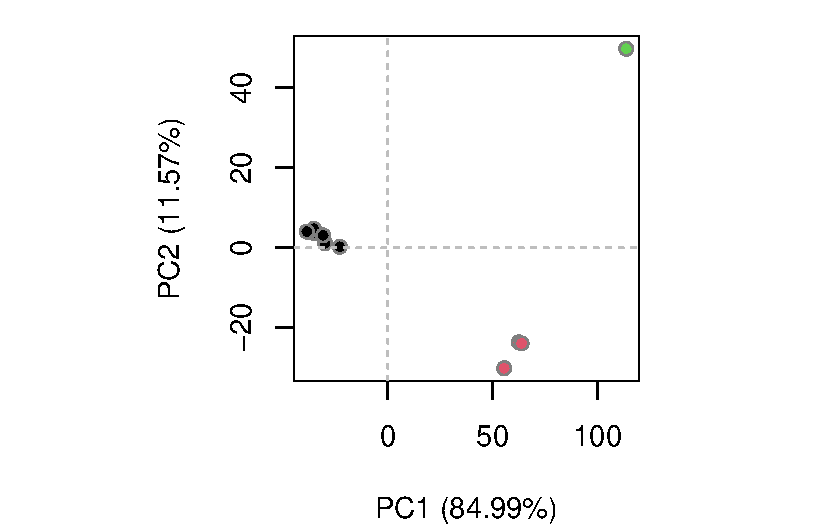
\includegraphics{Class11INCLASS_files/figure-pdf/unnamed-chunk-13-1.pdf}

}

\end{figure}

\#\#\#\#\#HOMEWORK \includegraphics{HIV_MONOMER.pdf}

\begin{Shaded}
\begin{Highlighting}[]
\NormalTok{results\_dir }\OtherTok{\textless{}{-}} \StringTok{"hivpr\_dimer\_23119"}
\end{Highlighting}
\end{Shaded}

\begin{Shaded}
\begin{Highlighting}[]
\CommentTok{\# File names for all PDB models}
\NormalTok{pdb\_files }\OtherTok{\textless{}{-}} \FunctionTok{list.files}\NormalTok{(}\AttributeTok{path=}\NormalTok{results\_dir,}
                        \AttributeTok{pattern=}\StringTok{"*.pdb"}\NormalTok{,}
                        \AttributeTok{full.names =} \ConstantTok{TRUE}\NormalTok{)}
\NormalTok{pdb\_files}
\end{Highlighting}
\end{Shaded}

\begin{verbatim}
[1] "hivpr_dimer_23119/hivpr_dimer_23119_unrelaxed_rank_001_alphafold2_multimer_v3_model_1_seed_000.pdb"
[2] "hivpr_dimer_23119/hivpr_dimer_23119_unrelaxed_rank_002_alphafold2_multimer_v3_model_5_seed_000.pdb"
[3] "hivpr_dimer_23119/hivpr_dimer_23119_unrelaxed_rank_003_alphafold2_multimer_v3_model_4_seed_000.pdb"
[4] "hivpr_dimer_23119/hivpr_dimer_23119_unrelaxed_rank_004_alphafold2_multimer_v3_model_2_seed_000.pdb"
[5] "hivpr_dimer_23119/hivpr_dimer_23119_unrelaxed_rank_005_alphafold2_multimer_v3_model_3_seed_000.pdb"
\end{verbatim}

\begin{Shaded}
\begin{Highlighting}[]
\FunctionTok{library}\NormalTok{(bio3d)}

\CommentTok{\# Read all data from Models }
\CommentTok{\#  and superpose/fit coords}
\NormalTok{pdbs }\OtherTok{\textless{}{-}} \FunctionTok{pdbaln}\NormalTok{(pdb\_files, }\AttributeTok{fit=}\ConstantTok{TRUE}\NormalTok{, }\AttributeTok{exefile=}\StringTok{"msa"}\NormalTok{)}
\end{Highlighting}
\end{Shaded}

\begin{verbatim}
Reading PDB files:
hivpr_dimer_23119/hivpr_dimer_23119_unrelaxed_rank_001_alphafold2_multimer_v3_model_1_seed_000.pdb
hivpr_dimer_23119/hivpr_dimer_23119_unrelaxed_rank_002_alphafold2_multimer_v3_model_5_seed_000.pdb
hivpr_dimer_23119/hivpr_dimer_23119_unrelaxed_rank_003_alphafold2_multimer_v3_model_4_seed_000.pdb
hivpr_dimer_23119/hivpr_dimer_23119_unrelaxed_rank_004_alphafold2_multimer_v3_model_2_seed_000.pdb
hivpr_dimer_23119/hivpr_dimer_23119_unrelaxed_rank_005_alphafold2_multimer_v3_model_3_seed_000.pdb
.....

Extracting sequences

pdb/seq: 1   name: hivpr_dimer_23119/hivpr_dimer_23119_unrelaxed_rank_001_alphafold2_multimer_v3_model_1_seed_000.pdb 
pdb/seq: 2   name: hivpr_dimer_23119/hivpr_dimer_23119_unrelaxed_rank_002_alphafold2_multimer_v3_model_5_seed_000.pdb 
pdb/seq: 3   name: hivpr_dimer_23119/hivpr_dimer_23119_unrelaxed_rank_003_alphafold2_multimer_v3_model_4_seed_000.pdb 
pdb/seq: 4   name: hivpr_dimer_23119/hivpr_dimer_23119_unrelaxed_rank_004_alphafold2_multimer_v3_model_2_seed_000.pdb 
pdb/seq: 5   name: hivpr_dimer_23119/hivpr_dimer_23119_unrelaxed_rank_005_alphafold2_multimer_v3_model_3_seed_000.pdb 
\end{verbatim}

\begin{Shaded}
\begin{Highlighting}[]
\NormalTok{pdbs}
\end{Highlighting}
\end{Shaded}

\begin{verbatim}
                               1        .         .         .         .         50 
[Truncated_Name:1]hivpr_dime   PQITLWQRPLVTIKIGGQLKEALLDTGADDTVLEEMSLPGRWKPKMIGGI
[Truncated_Name:2]hivpr_dime   PQITLWQRPLVTIKIGGQLKEALLDTGADDTVLEEMSLPGRWKPKMIGGI
[Truncated_Name:3]hivpr_dime   PQITLWQRPLVTIKIGGQLKEALLDTGADDTVLEEMSLPGRWKPKMIGGI
[Truncated_Name:4]hivpr_dime   PQITLWQRPLVTIKIGGQLKEALLDTGADDTVLEEMSLPGRWKPKMIGGI
[Truncated_Name:5]hivpr_dime   PQITLWQRPLVTIKIGGQLKEALLDTGADDTVLEEMSLPGRWKPKMIGGI
                               ************************************************** 
                               1        .         .         .         .         50 

                              51        .         .         .         .         100 
[Truncated_Name:1]hivpr_dime   GGFIKVRQYDQILIEICGHKAIGTVLVGPTPVNIIGRNLLTQIGCTLNFP
[Truncated_Name:2]hivpr_dime   GGFIKVRQYDQILIEICGHKAIGTVLVGPTPVNIIGRNLLTQIGCTLNFP
[Truncated_Name:3]hivpr_dime   GGFIKVRQYDQILIEICGHKAIGTVLVGPTPVNIIGRNLLTQIGCTLNFP
[Truncated_Name:4]hivpr_dime   GGFIKVRQYDQILIEICGHKAIGTVLVGPTPVNIIGRNLLTQIGCTLNFP
[Truncated_Name:5]hivpr_dime   GGFIKVRQYDQILIEICGHKAIGTVLVGPTPVNIIGRNLLTQIGCTLNFP
                               ************************************************** 
                              51        .         .         .         .         100 

                             101        .         .         .         .         150 
[Truncated_Name:1]hivpr_dime   QITLWQRPLVTIKIGGQLKEALLDTGADDTVLEEMSLPGRWKPKMIGGIG
[Truncated_Name:2]hivpr_dime   QITLWQRPLVTIKIGGQLKEALLDTGADDTVLEEMSLPGRWKPKMIGGIG
[Truncated_Name:3]hivpr_dime   QITLWQRPLVTIKIGGQLKEALLDTGADDTVLEEMSLPGRWKPKMIGGIG
[Truncated_Name:4]hivpr_dime   QITLWQRPLVTIKIGGQLKEALLDTGADDTVLEEMSLPGRWKPKMIGGIG
[Truncated_Name:5]hivpr_dime   QITLWQRPLVTIKIGGQLKEALLDTGADDTVLEEMSLPGRWKPKMIGGIG
                               ************************************************** 
                             101        .         .         .         .         150 

                             151        .         .         .         .       198 
[Truncated_Name:1]hivpr_dime   GFIKVRQYDQILIEICGHKAIGTVLVGPTPVNIIGRNLLTQIGCTLNF
[Truncated_Name:2]hivpr_dime   GFIKVRQYDQILIEICGHKAIGTVLVGPTPVNIIGRNLLTQIGCTLNF
[Truncated_Name:3]hivpr_dime   GFIKVRQYDQILIEICGHKAIGTVLVGPTPVNIIGRNLLTQIGCTLNF
[Truncated_Name:4]hivpr_dime   GFIKVRQYDQILIEICGHKAIGTVLVGPTPVNIIGRNLLTQIGCTLNF
[Truncated_Name:5]hivpr_dime   GFIKVRQYDQILIEICGHKAIGTVLVGPTPVNIIGRNLLTQIGCTLNF
                               ************************************************ 
                             151        .         .         .         .       198 

Call:
  pdbaln(files = pdb_files, fit = TRUE, exefile = "msa")

Class:
  pdbs, fasta

Alignment dimensions:
  5 sequence rows; 198 position columns (198 non-gap, 0 gap) 

+ attr: xyz, resno, b, chain, id, ali, resid, sse, call
\end{verbatim}

\begin{Shaded}
\begin{Highlighting}[]
\NormalTok{rd }\OtherTok{\textless{}{-}} \FunctionTok{rmsd}\NormalTok{(pdbs, }\AttributeTok{fit=}\NormalTok{T)}
\end{Highlighting}
\end{Shaded}

\begin{verbatim}
Warning in rmsd(pdbs, fit = T): No indices provided, using the 198 non NA positions
\end{verbatim}

\begin{Shaded}
\begin{Highlighting}[]
\FunctionTok{range}\NormalTok{(rd)}
\end{Highlighting}
\end{Shaded}

\begin{verbatim}
[1]  0.000 14.689
\end{verbatim}

\begin{Shaded}
\begin{Highlighting}[]
\CommentTok{\#install.packages("pheatmap)}
\FunctionTok{library}\NormalTok{(pheatmap)}

\FunctionTok{colnames}\NormalTok{(rd) }\OtherTok{\textless{}{-}} \FunctionTok{paste0}\NormalTok{(}\StringTok{"m"}\NormalTok{,}\DecValTok{1}\SpecialCharTok{:}\DecValTok{5}\NormalTok{)}
\FunctionTok{rownames}\NormalTok{(rd) }\OtherTok{\textless{}{-}} \FunctionTok{paste0}\NormalTok{(}\StringTok{"m"}\NormalTok{,}\DecValTok{1}\SpecialCharTok{:}\DecValTok{5}\NormalTok{)}
\FunctionTok{pheatmap}\NormalTok{(rd)}
\end{Highlighting}
\end{Shaded}

\begin{figure}[H]

{\centering 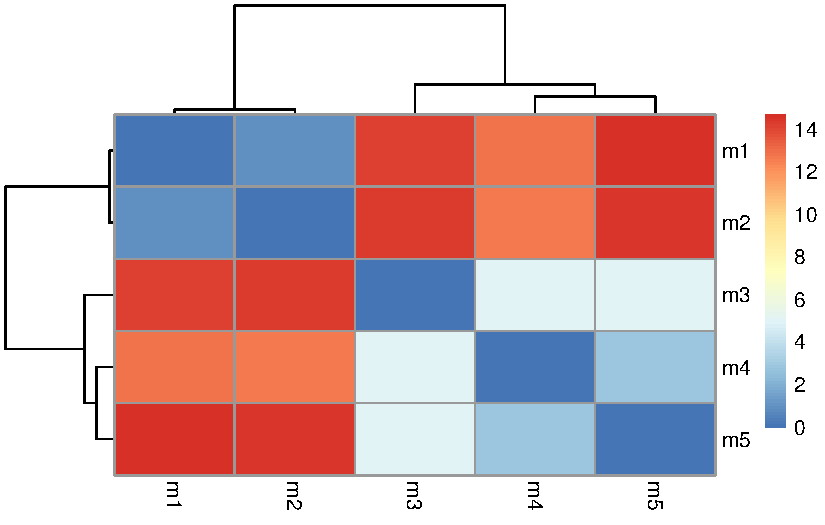
\includegraphics{Class11INCLASS_files/figure-pdf/unnamed-chunk-19-1.pdf}

}

\end{figure}

\begin{Shaded}
\begin{Highlighting}[]
\CommentTok{\# Read a reference PDB structure}
\NormalTok{pdb }\OtherTok{\textless{}{-}} \FunctionTok{read.pdb}\NormalTok{(}\StringTok{"1hsg"}\NormalTok{)}
\end{Highlighting}
\end{Shaded}

\begin{verbatim}
  Note: Accessing on-line PDB file
\end{verbatim}

\begin{Shaded}
\begin{Highlighting}[]
\FunctionTok{plotb3}\NormalTok{(pdbs}\SpecialCharTok{$}\NormalTok{b[}\DecValTok{1}\NormalTok{,], }\AttributeTok{typ=}\StringTok{"l"}\NormalTok{, }\AttributeTok{lwd=}\DecValTok{2}\NormalTok{, }\AttributeTok{sse=}\NormalTok{pdb)}
\FunctionTok{points}\NormalTok{(pdbs}\SpecialCharTok{$}\NormalTok{b[}\DecValTok{2}\NormalTok{,], }\AttributeTok{typ=}\StringTok{"l"}\NormalTok{, }\AttributeTok{col=}\StringTok{"red"}\NormalTok{)}
\FunctionTok{points}\NormalTok{(pdbs}\SpecialCharTok{$}\NormalTok{b[}\DecValTok{3}\NormalTok{,], }\AttributeTok{typ=}\StringTok{"l"}\NormalTok{, }\AttributeTok{col=}\StringTok{"blue"}\NormalTok{)}
\FunctionTok{points}\NormalTok{(pdbs}\SpecialCharTok{$}\NormalTok{b[}\DecValTok{4}\NormalTok{,], }\AttributeTok{typ=}\StringTok{"l"}\NormalTok{, }\AttributeTok{col=}\StringTok{"darkgreen"}\NormalTok{)}
\FunctionTok{points}\NormalTok{(pdbs}\SpecialCharTok{$}\NormalTok{b[}\DecValTok{5}\NormalTok{,], }\AttributeTok{typ=}\StringTok{"l"}\NormalTok{, }\AttributeTok{col=}\StringTok{"orange"}\NormalTok{)}
\FunctionTok{abline}\NormalTok{(}\AttributeTok{v=}\DecValTok{100}\NormalTok{, }\AttributeTok{col=}\StringTok{"gray"}\NormalTok{)}
\end{Highlighting}
\end{Shaded}

\begin{figure}[H]

{\centering 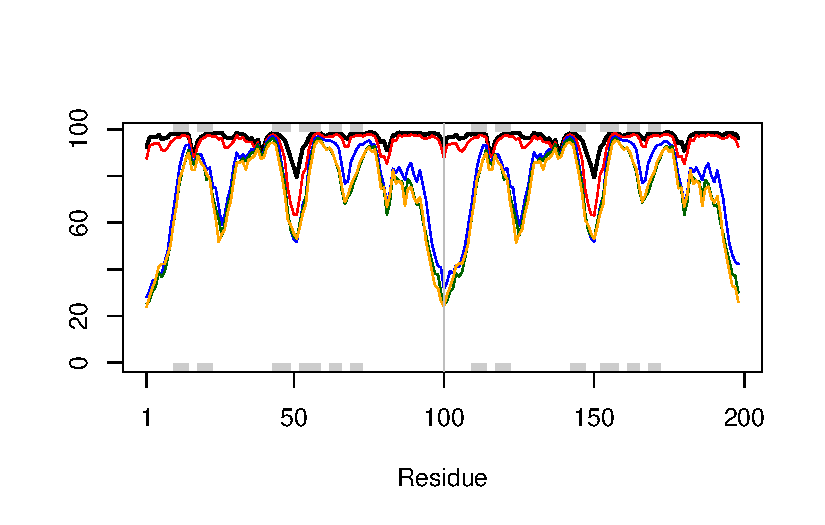
\includegraphics{Class11INCLASS_files/figure-pdf/unnamed-chunk-21-1.pdf}

}

\end{figure}

\begin{Shaded}
\begin{Highlighting}[]
\NormalTok{core }\OtherTok{\textless{}{-}} \FunctionTok{core.find}\NormalTok{(pdbs)}
\end{Highlighting}
\end{Shaded}

\begin{verbatim}
 core size 197 of 198  vol = 6154.839 
 core size 196 of 198  vol = 5399.676 
 core size 195 of 198  vol = 5074.795 
 core size 194 of 198  vol = 4802.518 
 core size 193 of 198  vol = 4520.256 
 core size 192 of 198  vol = 4305.362 
 core size 191 of 198  vol = 4089.792 
 core size 190 of 198  vol = 3886.145 
 core size 189 of 198  vol = 3758.321 
 core size 188 of 198  vol = 3620.18 
 core size 187 of 198  vol = 3496.698 
 core size 186 of 198  vol = 3389.985 
 core size 185 of 198  vol = 3320.114 
 core size 184 of 198  vol = 3258.683 
 core size 183 of 198  vol = 3208.591 
 core size 182 of 198  vol = 3156.736 
 core size 181 of 198  vol = 3141.668 
 core size 180 of 198  vol = 3136.574 
 core size 179 of 198  vol = 3155.52 
 core size 178 of 198  vol = 3185.362 
 core size 177 of 198  vol = 3204.487 
 core size 176 of 198  vol = 3211.978 
 core size 175 of 198  vol = 3234.993 
 core size 174 of 198  vol = 3244.062 
 core size 173 of 198  vol = 3237.845 
 core size 172 of 198  vol = 3218.77 
 core size 171 of 198  vol = 3180.743 
 core size 170 of 198  vol = 3130.369 
 core size 169 of 198  vol = 3067.881 
 core size 168 of 198  vol = 2989.546 
 core size 167 of 198  vol = 2928.272 
 core size 166 of 198  vol = 2851.193 
 core size 165 of 198  vol = 2780.877 
 core size 164 of 198  vol = 2708.433 
 core size 163 of 198  vol = 2636.516 
 core size 162 of 198  vol = 2563.25 
 core size 161 of 198  vol = 2478.024 
 core size 160 of 198  vol = 2404.793 
 core size 159 of 198  vol = 2330.997 
 core size 158 of 198  vol = 2250.477 
 core size 157 of 198  vol = 2159.432 
 core size 156 of 198  vol = 2070.759 
 core size 155 of 198  vol = 1983.579 
 core size 154 of 198  vol = 1917.913 
 core size 153 of 198  vol = 1842.556 
 core size 152 of 198  vol = 1775.398 
 core size 151 of 198  vol = 1695.133 
 core size 150 of 198  vol = 1632.173 
 core size 149 of 198  vol = 1570.391 
 core size 148 of 198  vol = 1497.238 
 core size 147 of 198  vol = 1434.802 
 core size 146 of 198  vol = 1367.706 
 core size 145 of 198  vol = 1302.596 
 core size 144 of 198  vol = 1251.985 
 core size 143 of 198  vol = 1207.976 
 core size 142 of 198  vol = 1167.112 
 core size 141 of 198  vol = 1118.27 
 core size 140 of 198  vol = 1081.664 
 core size 139 of 198  vol = 1029.75 
 core size 138 of 198  vol = 981.766 
 core size 137 of 198  vol = 944.446 
 core size 136 of 198  vol = 899.224 
 core size 135 of 198  vol = 859.402 
 core size 134 of 198  vol = 814.694 
 core size 133 of 198  vol = 771.862 
 core size 132 of 198  vol = 733.807 
 core size 131 of 198  vol = 702.053 
 core size 130 of 198  vol = 658.757 
 core size 129 of 198  vol = 622.574 
 core size 128 of 198  vol = 578.29 
 core size 127 of 198  vol = 543.07 
 core size 126 of 198  vol = 510.934 
 core size 125 of 198  vol = 481.595 
 core size 124 of 198  vol = 464.672 
 core size 123 of 198  vol = 451.721 
 core size 122 of 198  vol = 430.417 
 core size 121 of 198  vol = 409.141 
 core size 120 of 198  vol = 378.942 
 core size 119 of 198  vol = 348.325 
 core size 118 of 198  vol = 324.738 
 core size 117 of 198  vol = 312.394 
 core size 116 of 198  vol = 300.89 
 core size 115 of 198  vol = 279.976 
 core size 114 of 198  vol = 263.434 
 core size 113 of 198  vol = 250.263 
 core size 112 of 198  vol = 229.592 
 core size 111 of 198  vol = 209.929 
 core size 110 of 198  vol = 196.379 
 core size 109 of 198  vol = 180.628 
 core size 108 of 198  vol = 167.088 
 core size 107 of 198  vol = 155.875 
 core size 106 of 198  vol = 142.595 
 core size 105 of 198  vol = 128.924 
 core size 104 of 198  vol = 114.054 
 core size 103 of 198  vol = 100.936 
 core size 102 of 198  vol = 90.431 
 core size 101 of 198  vol = 81.972 
 core size 100 of 198  vol = 74.017 
 core size 99 of 198  vol = 66.855 
 core size 98 of 198  vol = 59.525 
 core size 97 of 198  vol = 52.263 
 core size 96 of 198  vol = 43.699 
 core size 95 of 198  vol = 35.813 
 core size 94 of 198  vol = 28.888 
 core size 93 of 198  vol = 20.692 
 core size 92 of 198  vol = 14.975 
 core size 91 of 198  vol = 9.146 
 core size 90 of 198  vol = 5.232 
 core size 89 of 198  vol = 3.53 
 core size 88 of 198  vol = 2.657 
 core size 87 of 198  vol = 1.998 
 core size 86 of 198  vol = 1.333 
 core size 85 of 198  vol = 1.141 
 core size 84 of 198  vol = 1.012 
 core size 83 of 198  vol = 0.891 
 core size 82 of 198  vol = 0.749 
 core size 81 of 198  vol = 0.618 
 core size 80 of 198  vol = 0.538 
 core size 79 of 198  vol = 0.479 
 FINISHED: Min vol ( 0.5 ) reached
\end{verbatim}

\begin{Shaded}
\begin{Highlighting}[]
\NormalTok{core.inds }\OtherTok{\textless{}{-}} \FunctionTok{print}\NormalTok{(core, }\AttributeTok{vol=}\FloatTok{0.5}\NormalTok{)}
\end{Highlighting}
\end{Shaded}

\begin{verbatim}
# 80 positions (cumulative volume <= 0.5 Angstrom^3) 
  start end length
1    10  25     16
2    27  48     22
3    53  94     42
\end{verbatim}

\begin{Shaded}
\begin{Highlighting}[]
\NormalTok{xyz }\OtherTok{\textless{}{-}} \FunctionTok{pdbfit}\NormalTok{(pdbs, core.inds, }\AttributeTok{outpath=}\StringTok{"corefit\_structures"}\NormalTok{)}
\end{Highlighting}
\end{Shaded}

\hypertarget{section}{%
\section{}\label{section}}

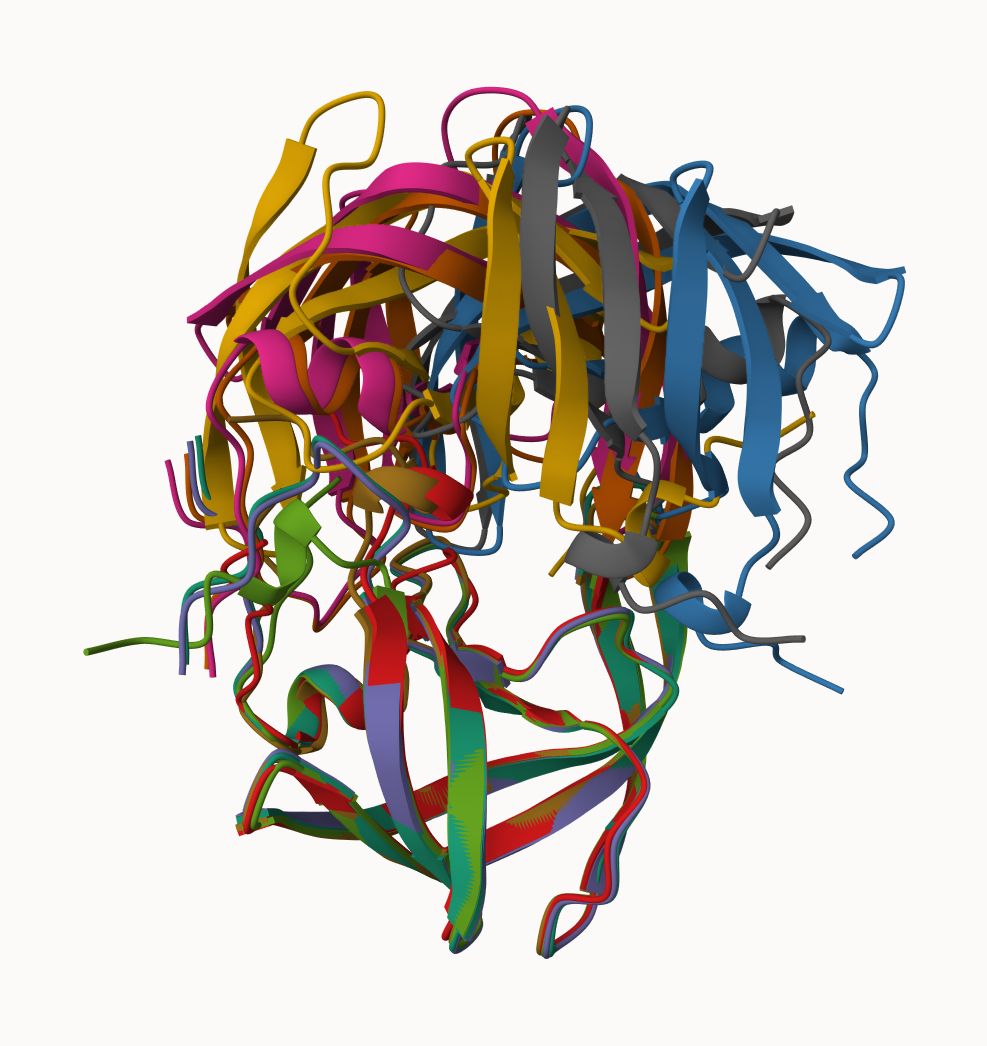
\includegraphics{HIVPR_DIMER_23119.pdf}

\begin{Shaded}
\begin{Highlighting}[]
\NormalTok{rf }\OtherTok{\textless{}{-}} \FunctionTok{rmsf}\NormalTok{(xyz)}

\FunctionTok{plotb3}\NormalTok{(rf, }\AttributeTok{sse=}\NormalTok{pdb)}
\FunctionTok{abline}\NormalTok{(}\AttributeTok{v=}\DecValTok{100}\NormalTok{, }\AttributeTok{col=}\StringTok{"gray"}\NormalTok{, }\AttributeTok{ylab=}\StringTok{"RMSF"}\NormalTok{)}
\end{Highlighting}
\end{Shaded}

\begin{figure}[H]

{\centering 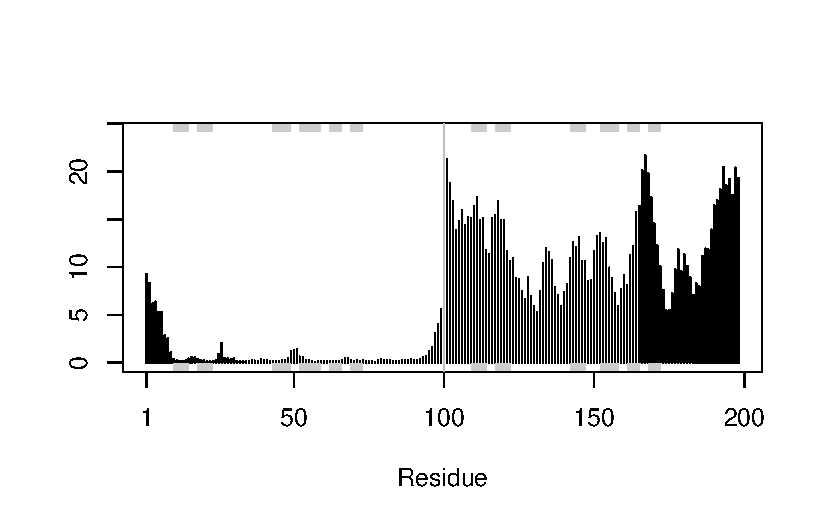
\includegraphics{Class11INCLASS_files/figure-pdf/unnamed-chunk-25-1.pdf}

}

\end{figure}

\begin{Shaded}
\begin{Highlighting}[]
\FunctionTok{library}\NormalTok{(jsonlite)}

\CommentTok{\# Listing of all PAE JSON files}
\NormalTok{pae\_files }\OtherTok{\textless{}{-}} \FunctionTok{list.files}\NormalTok{(}\AttributeTok{path=}\NormalTok{results\_dir,}
                        \AttributeTok{pattern=}\StringTok{".*model.*}\SpecialCharTok{\textbackslash{}\textbackslash{}}\StringTok{.json"}\NormalTok{,}
                        \AttributeTok{full.names =} \ConstantTok{TRUE}\NormalTok{)}
\end{Highlighting}
\end{Shaded}

\begin{Shaded}
\begin{Highlighting}[]
\NormalTok{pae1 }\OtherTok{\textless{}{-}} \FunctionTok{read\_json}\NormalTok{(pae\_files[}\DecValTok{1}\NormalTok{],}\AttributeTok{simplifyVector =} \ConstantTok{TRUE}\NormalTok{)}
\NormalTok{pae5 }\OtherTok{\textless{}{-}} \FunctionTok{read\_json}\NormalTok{(pae\_files[}\DecValTok{5}\NormalTok{],}\AttributeTok{simplifyVector =} \ConstantTok{TRUE}\NormalTok{)}

\FunctionTok{attributes}\NormalTok{(pae1)}
\end{Highlighting}
\end{Shaded}

\begin{verbatim}
$names
[1] "plddt"   "max_pae" "pae"     "ptm"     "iptm"   
\end{verbatim}

\begin{Shaded}
\begin{Highlighting}[]
\CommentTok{\# Per{-}residue pLDDT scores }
\CommentTok{\#  same as B{-}factor of PDB..}
\FunctionTok{head}\NormalTok{(pae1}\SpecialCharTok{$}\NormalTok{plddt) }
\end{Highlighting}
\end{Shaded}

\begin{verbatim}
[1] 92.50 96.56 96.94 96.62 97.69 96.00
\end{verbatim}

\begin{Shaded}
\begin{Highlighting}[]
\NormalTok{pae1}\SpecialCharTok{$}\NormalTok{max\_pae}
\end{Highlighting}
\end{Shaded}

\begin{verbatim}
[1] 15.54688
\end{verbatim}

\begin{Shaded}
\begin{Highlighting}[]
\NormalTok{pae5}\SpecialCharTok{$}\NormalTok{max\_pae}
\end{Highlighting}
\end{Shaded}

\begin{verbatim}
[1] 29.29688
\end{verbatim}

\begin{Shaded}
\begin{Highlighting}[]
\FunctionTok{plot.dmat}\NormalTok{(pae1}\SpecialCharTok{$}\NormalTok{pae, }
          \AttributeTok{xlab=}\StringTok{"Residue Position (i)"}\NormalTok{,}
          \AttributeTok{ylab=}\StringTok{"Residue Position (j)"}\NormalTok{)}
\end{Highlighting}
\end{Shaded}

\begin{figure}[H]

{\centering 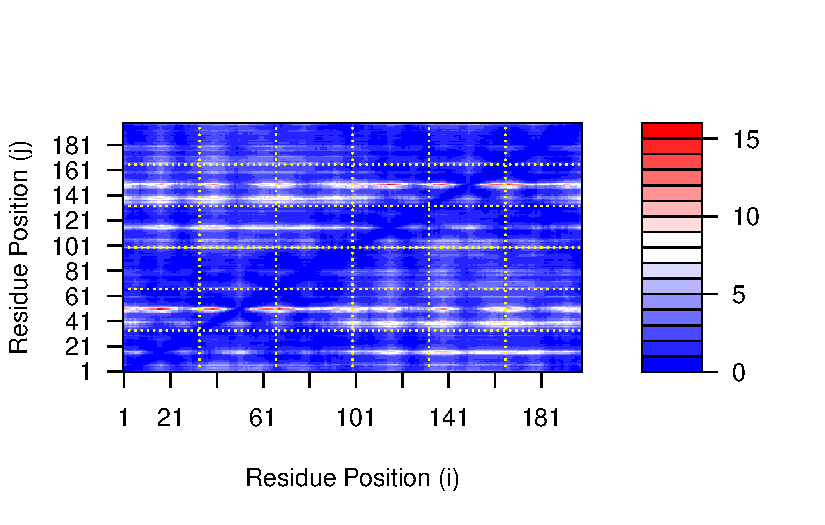
\includegraphics{Class11INCLASS_files/figure-pdf/unnamed-chunk-31-1.pdf}

}

\end{figure}

\begin{Shaded}
\begin{Highlighting}[]
\FunctionTok{plot.dmat}\NormalTok{(pae5}\SpecialCharTok{$}\NormalTok{pae, }
          \AttributeTok{xlab=}\StringTok{"Residue Position (i)"}\NormalTok{,}
          \AttributeTok{ylab=}\StringTok{"Residue Position (j)"}\NormalTok{,}
          \AttributeTok{grid.col =} \StringTok{"black"}\NormalTok{,}
          \AttributeTok{zlim=}\FunctionTok{c}\NormalTok{(}\DecValTok{0}\NormalTok{,}\DecValTok{30}\NormalTok{))}
\end{Highlighting}
\end{Shaded}

\begin{figure}[H]

{\centering 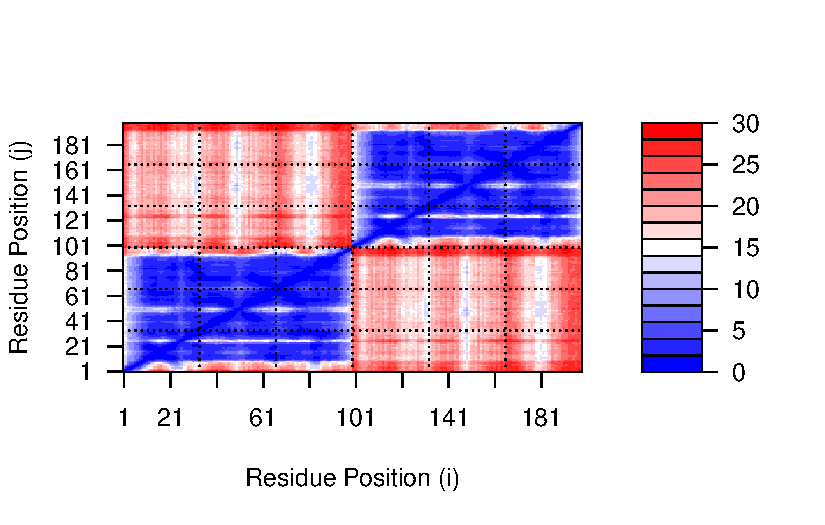
\includegraphics{Class11INCLASS_files/figure-pdf/unnamed-chunk-32-1.pdf}

}

\end{figure}

\begin{Shaded}
\begin{Highlighting}[]
\FunctionTok{plot.dmat}\NormalTok{(pae1}\SpecialCharTok{$}\NormalTok{pae, }
          \AttributeTok{xlab=}\StringTok{"Residue Position (i)"}\NormalTok{,}
          \AttributeTok{ylab=}\StringTok{"Residue Position (j)"}\NormalTok{,}
          \AttributeTok{grid.col =} \StringTok{"black"}\NormalTok{,}
          \AttributeTok{zlim=}\FunctionTok{c}\NormalTok{(}\DecValTok{0}\NormalTok{,}\DecValTok{30}\NormalTok{))}
\end{Highlighting}
\end{Shaded}

\begin{figure}[H]

{\centering 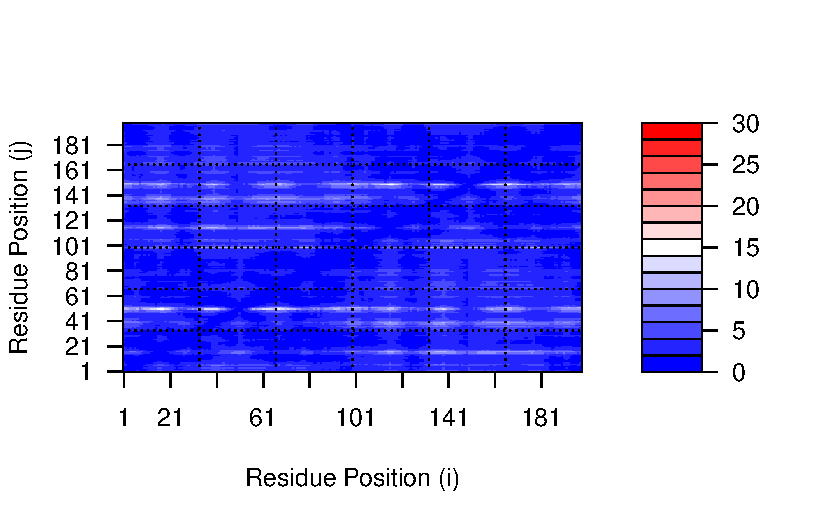
\includegraphics{Class11INCLASS_files/figure-pdf/unnamed-chunk-33-1.pdf}

}

\end{figure}

\begin{Shaded}
\begin{Highlighting}[]
\NormalTok{aln\_file }\OtherTok{\textless{}{-}} \FunctionTok{list.files}\NormalTok{(}\AttributeTok{path=}\NormalTok{results\_dir,}
                       \AttributeTok{pattern=}\StringTok{".a3m$"}\NormalTok{,}
                        \AttributeTok{full.names =} \ConstantTok{TRUE}\NormalTok{)}
\NormalTok{aln\_file}
\end{Highlighting}
\end{Shaded}

\begin{verbatim}
[1] "hivpr_dimer_23119/hivpr_dimer_23119.a3m"
\end{verbatim}

\begin{Shaded}
\begin{Highlighting}[]
\NormalTok{aln }\OtherTok{\textless{}{-}} \FunctionTok{read.fasta}\NormalTok{(aln\_file[}\DecValTok{1}\NormalTok{], }\AttributeTok{to.upper =} \ConstantTok{TRUE}\NormalTok{)}
\end{Highlighting}
\end{Shaded}

\begin{verbatim}
[1] " ** Duplicated sequence id's: 101 **"
[2] " ** Duplicated sequence id's: 101 **"
\end{verbatim}

\begin{Shaded}
\begin{Highlighting}[]
\FunctionTok{dim}\NormalTok{(aln}\SpecialCharTok{$}\NormalTok{ali)}
\end{Highlighting}
\end{Shaded}

\begin{verbatim}
[1] 5378  132
\end{verbatim}

\begin{Shaded}
\begin{Highlighting}[]
\NormalTok{sim }\OtherTok{\textless{}{-}} \FunctionTok{conserv}\NormalTok{(aln)}
\end{Highlighting}
\end{Shaded}

\begin{Shaded}
\begin{Highlighting}[]
\FunctionTok{plotb3}\NormalTok{(sim[}\DecValTok{1}\SpecialCharTok{:}\DecValTok{99}\NormalTok{], }\AttributeTok{sse=}\FunctionTok{trim.pdb}\NormalTok{(pdb, }\AttributeTok{chain=}\StringTok{"A"}\NormalTok{),}
       \AttributeTok{ylab=}\StringTok{"Conservation Score"}\NormalTok{)}
\end{Highlighting}
\end{Shaded}

\begin{figure}[H]

{\centering 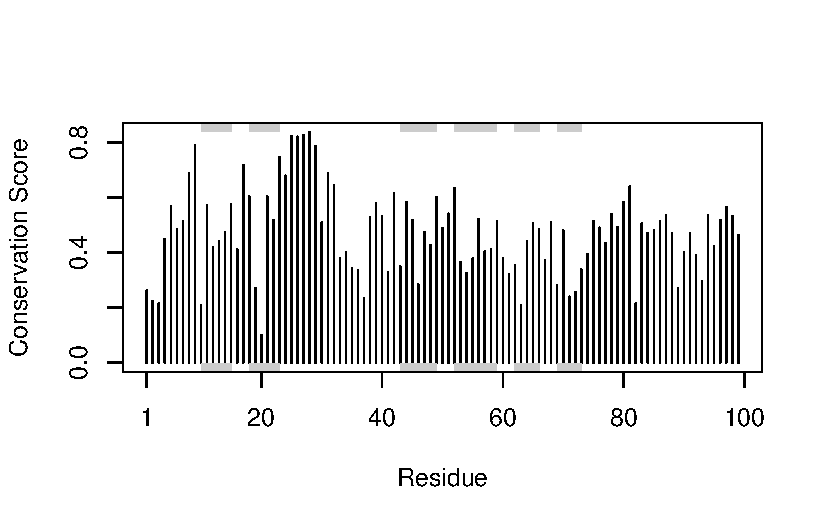
\includegraphics{Class11INCLASS_files/figure-pdf/unnamed-chunk-38-1.pdf}

}

\end{figure}

\begin{Shaded}
\begin{Highlighting}[]
\NormalTok{con }\OtherTok{\textless{}{-}} \FunctionTok{consensus}\NormalTok{(aln, }\AttributeTok{cutoff =} \FloatTok{0.9}\NormalTok{)}
\NormalTok{con}\SpecialCharTok{$}\NormalTok{seq}
\end{Highlighting}
\end{Shaded}

\begin{verbatim}
  [1] "-" "-" "-" "-" "-" "-" "-" "-" "-" "-" "-" "-" "-" "-" "-" "-" "-" "-"
 [19] "-" "-" "-" "-" "-" "-" "D" "T" "G" "A" "-" "-" "-" "-" "-" "-" "-" "-"
 [37] "-" "-" "-" "-" "-" "-" "-" "-" "-" "-" "-" "-" "-" "-" "-" "-" "-" "-"
 [55] "-" "-" "-" "-" "-" "-" "-" "-" "-" "-" "-" "-" "-" "-" "-" "-" "-" "-"
 [73] "-" "-" "-" "-" "-" "-" "-" "-" "-" "-" "-" "-" "-" "-" "-" "-" "-" "-"
 [91] "-" "-" "-" "-" "-" "-" "-" "-" "-" "-" "-" "-" "-" "-" "-" "-" "-" "-"
[109] "-" "-" "-" "-" "-" "-" "-" "-" "-" "-" "-" "-" "-" "-" "-" "-" "-" "-"
[127] "-" "-" "-" "-" "-" "-"
\end{verbatim}

\begin{Shaded}
\begin{Highlighting}[]
\NormalTok{m1.pdb }\OtherTok{\textless{}{-}} \FunctionTok{read.pdb}\NormalTok{(pdb\_files[}\DecValTok{1}\NormalTok{])}
\NormalTok{occ }\OtherTok{\textless{}{-}} \FunctionTok{vec2resno}\NormalTok{(}\FunctionTok{c}\NormalTok{(sim[}\DecValTok{1}\SpecialCharTok{:}\DecValTok{99}\NormalTok{], sim[}\DecValTok{1}\SpecialCharTok{:}\DecValTok{99}\NormalTok{]), m1.pdb}\SpecialCharTok{$}\NormalTok{atom}\SpecialCharTok{$}\NormalTok{resno)}
\FunctionTok{write.pdb}\NormalTok{(m1.pdb, }\AttributeTok{o=}\NormalTok{occ, }\AttributeTok{file=}\StringTok{"m1\_conserv.pdb"}\NormalTok{)}
\end{Highlighting}
\end{Shaded}




\end{document}
